\section{Misurazione della pressione di vapore dell'acqua a temperature differenti}

%In questa sezione illustreremo il materiale a nostra disposizione per l'esecuzione
%dell'esperimento e di seguito faremo un'analisi dei dati da noi raccolti.

\subsection{Apparato sperimentale}

Il materiale a nostra disposizione è il seguente:
\begin{itemize}
	\item{Riscaldatore con agitatore magnetico;}
	\item{Termometro ad alcohol con una risoluzione di misura di 1$^\circ$C;}
	\item{Manometro di Bourdon con una risoluzione di misura di 5000 Pa;}
	\item{Apparato per la misura della pressione di vapore, consistente in un beaker,
    in una bottiglietta di vetro con tappo sigillante, un sostegno per l'apparato, acqua distillata e raccorderia varia;}
\end{itemize}

\subsection{Raccolta dati}

Per misurare la pressione di vapore dell'acqua a differenti temperature abbiamo adottato questo procedimento:

\begin{itemize}
	\item{abbiamo posto a bagnomaria la bottigietta di vetro;}
	\item{abbiamo fatto raggiungere la temperatura di circa 20$^\circ$C all'acqua demineralizzata interna alla bottiglietta;}
	\item{variando la pressione interna della bottiglietta abbiamo riempito il
        tubicino che collega la bottiglia con il manometro di acqua, che è un fluido incomprimibile;}
	\item{una volta che il sistema ha raggiunto la temperatura di 35$^\circ$C abbiamo
        iniziato a raccogliere i dati leggendo per ogni variazione della pressione pari
        a 5 kPa, la corrispettiva temperatura dell'acqua nella bottiglia;}
	\item{il processo è stato interrotto una volta raggiunta una temperatura interna di
        circa 85$^\circ$C. A questo punto non si è più somministrata energia al sistema e sono
        stati raccolti i dati in discesa, ovvero man mano che il sistema andava raffreddandosi;}
\end{itemize}

\begin{figure}[h!]
    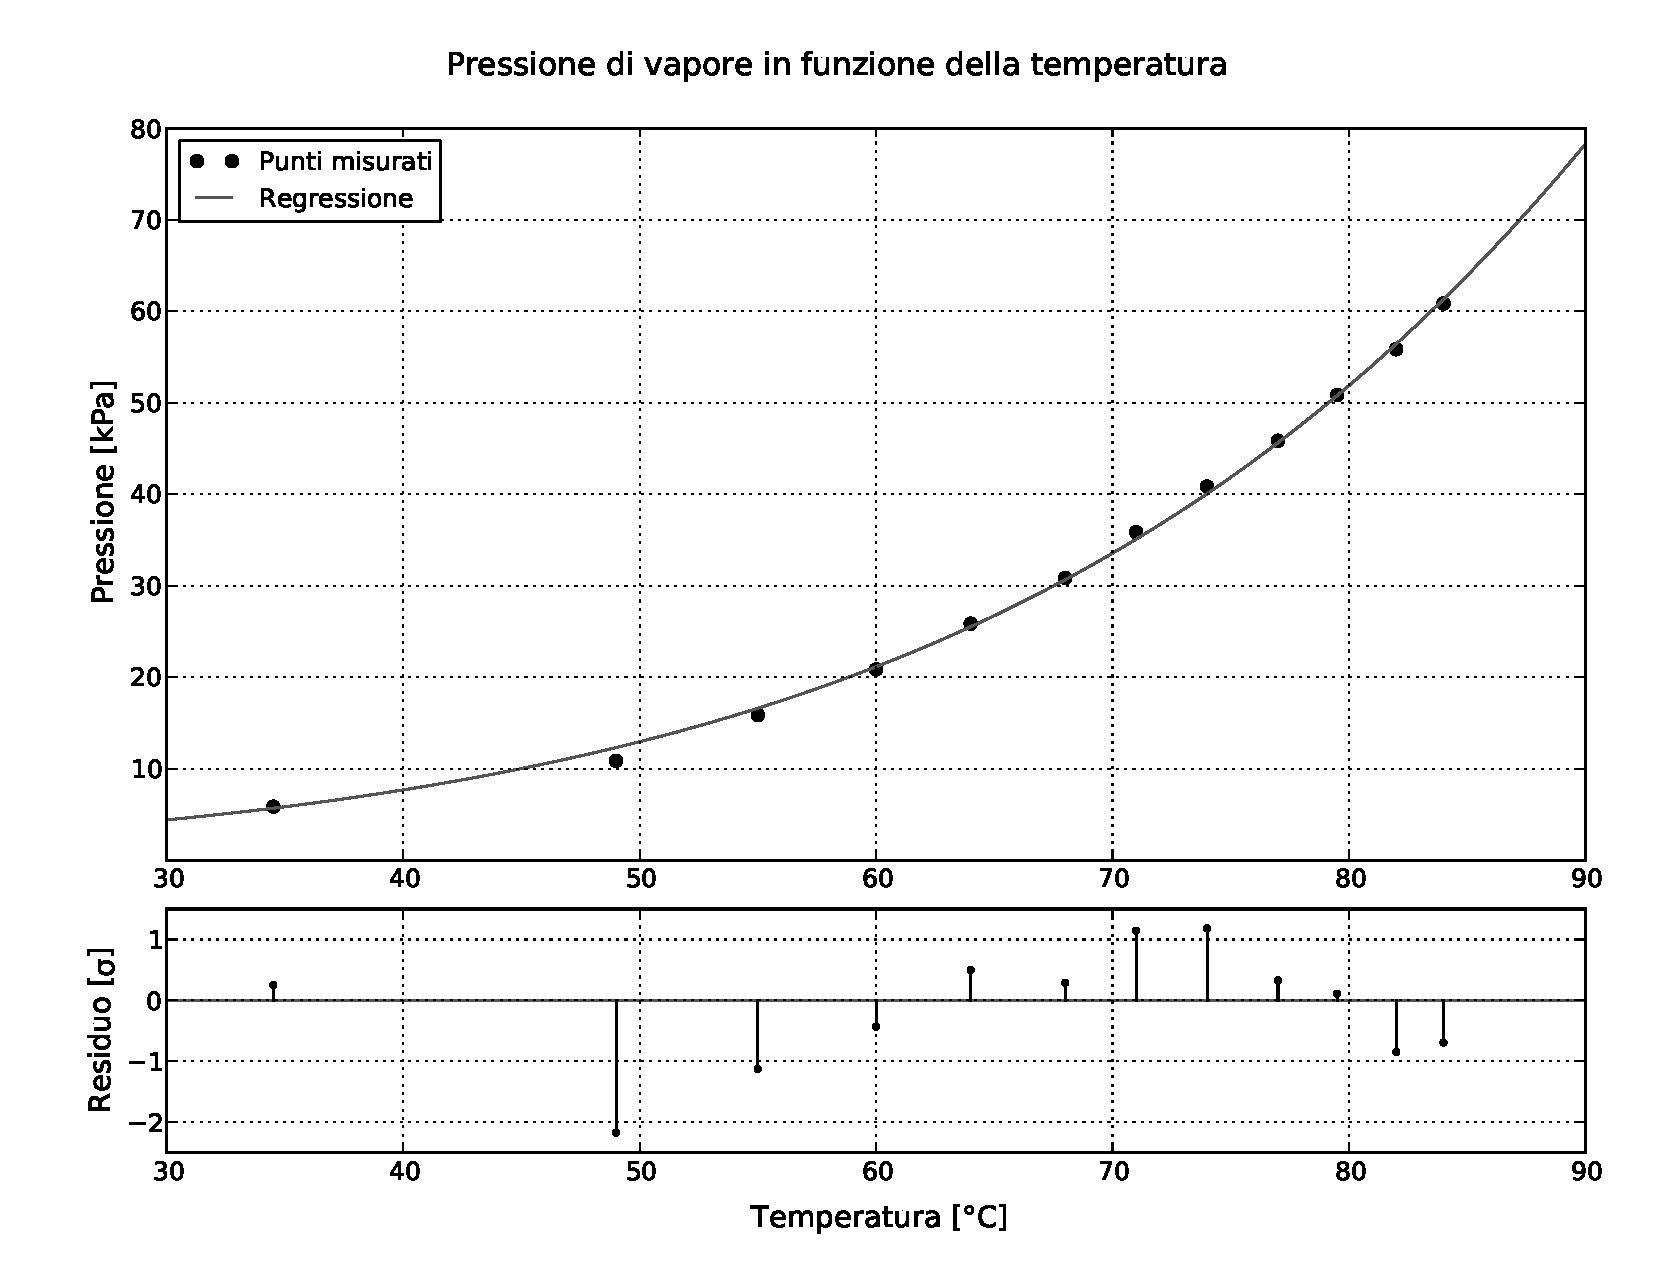
\includegraphics[width=16cm]{graph.pdf}
    \caption{Il grafico mostra i dati raccolti con la relativa incertezza. I dati seguono bene
    l'andamento tipico della pressione di vapore in funzione della temperatura.
    La curva tracciata è stata ottenuta con il metodo dei minimi quadrati. Le barre d'errore non sono
    mostrate in quanto comparabili con la dimensione dei punti sul grafico. Il grafico piccolo in basso
    mostra i residui (normalizzati col relativo errore), rispetto alla curva trovata.}
    \label{fig:graph}
\end{figure}


\subsection{Analisi dei dati}

L'equazione di Clapeyron può essere scritta nel seguente modo:

\begin{equation}
    P = P_0 \exp \left( - \frac{\Delta H}{RT} \right)
    \label{eq:clap}
\end{equation}
%
dove $P$ indica la pressione di vapore, $P_0$ è un parametro, $\Delta H$ è l'entalpia
(o calore latente) di vaporizzazione della sostanza in esame, $R$ è la costante dei gas, $T$ la temperatura.

Questa equazione descrive quindi il variare della pressione di vapore di una sostanza al variare della temperatura.
Per verificare questa legge abbiamo quindi misurato la pressione di vapore dell'acqua a diverse temperature,
ottenendo il grafico in Figura \ref{fig:graph}. 

Applicando il logaritmo ad entrambi i membri abbiamo linearizzato l'equazione (\ref{eq:clap}) ed eseguito la regressione lineare ottenendo i seguenti valori per i parametri:

\begin{equation}
    P_0 = 1.6 \cdot 10^{11} \pm 0.4 \cdot 10^{11} \; \si{\pascal} \qquad \Delta H = 43900 \pm  700 \; \si{\joule\per\kilo\gram} 
\end{equation}

Il valore di $P_0$ è poco interessante in quanto si tratta di un semplice parametro, al contrario il valore
$\Delta H$ ha un significato fisico preciso. Si tratta unfatti della quantità di energia necessaria a far evaporare un kilogrammo
di acqua. Il valore da noi trovato è in accordo con i valori reperibili in letteratura. Dobbiamo tuttavia specificare che il calore latente di vaporizzazione varia leggermente con la temperatura,
fatto non contemplato dai nostri calcoli.

La Figura \ref{fig:graph} riassume i risultati fin qui ottenuti. I dati sperimentali risultano in buon accordo
con la legge studiata. In particolare le incertezze da noi assunte si sono rivelate soprastimate, infatti
il chi quadro è risultato basso, e pertanto abbiamo dovuto corregerle. Quanto avvenuto ha senso poiché sul manometro potevamo facilmente
leggere variazioni di pressione di metà tacca (pari a 2500 \si{\pascal}).


\subsubsection{Calcolo della temperatura di ebbollizione dell'acqua}

Con i dati in nostro possesso siamo in grado di stimare la temperatura di ebbollizione dell'acqua.
Questo di per se non è uno degli scopi dell'esperimento, in quanto una misura diretta sarebbe molto
più semplice e precisa, tuttavia ci permette di controllare ulteriormente la correttezza dei calcoli
eseguiti e la ``bontà'' dell'esperimento.

La temperatura di ebbollizione di una sostanza è uguale alla temperatura in cui la pressione di vapore
è uguale alla pressione atmosferica. Noi abbiamo misurato una pressione atmosferica di:

\begin{equation}
    P\ped{atm} =  95900 \pm 100 \; \si{\pascal}
\end{equation}

Imponendo che la pressione di vapore dell'acqua (equazione (\ref{eq:clap})) sia uguale a $P\ped{atm}$, si ottiene:

\begin{equation}
    P\ped{atm} =  P_0 \exp \left( - \frac{\Delta H}{RT} \right) 
        \quad \implies \quad
    \log (P\ped{atm}) = \log (P_0) - \frac{\Delta H}{RT}
\end{equation}

Con due semplici passaggi algebrici si ottiene:

\begin{equation}
    T\ped{ebb} = T = \frac{\Delta H}{R(\log (P\ped{atm}) + \log (P_0))}
\end{equation}

Inserendo i valori numerici ricavati dai dati e propagando l'incertezza si ottiene

\begin{equation}
    T\ped{ebb} = 368 \pm 8 \; \si{\kelvin} = 95 \pm 8 \; \si{\celsius}
\end{equation}
%
che, tenendo conto del fatto che il luogo dove abbiamo eseguito l'esperimento è ad una quota di circa 350 m
sul livello del mare, è un risultato impreciso ma tuttavia corretto. L'altitudine infatti influisce sulla pressione atmosferica
abbassando la temperatura di ebbollizione dell'acqua.
